\documentclass[12pt, letterpaper]{article}
\usepackage{multicol}
\usepackage{natbib}
\usepackage{titling}
\usepackage{graphicx}
\graphicspath{{images/}}
\usepackage[toc,page]{appendix}
\usepackage{subcaption}
\usepackage{float}
\setlength{\columnsep}{0.6cm}
\usepackage[margin=1.2in]{geometry}
\title{}
\author{William Ewart}
\date{March 2017}

\begin{document}
\begin{titlingpage}
\maketitle
\tableofcontents
\end{titlingpage}
\newpage
\begin{multicols}{2}
\section{Introduction}
This paper uses spatial and cognitive agents to simulate social behaviours of a population with altruistic members. Replicating one of \cite{Powell} experiments showing that with increasing migratory levels the overall skill accumulation of a population increases. The code used to simulate this hypothesis is written in NetLogo and the same code used in \cite{Cace} paper on agent based communication. The results show that as the migratory distance increases the overall knowledge of the population increases however there is a certain point where the overall knowledge of the population is lower even though the migratory distance of the agents has increased. 
\section{Approach}
The code provided had all of the functionality that was required to run a suitable simulation with spacial and cognitive agents. The decision to measure the knowledge of the population depending on migration distance came from reading the \citep{Powell} paper. In his paper however he measures this against differing population densities rather than differing migration distances. The change in migration distances can show further details that affect the knowledge of a population. The only change made reported the knowledge of each turtle. This was necessary so that the behaviour space functionality within NetLogo could be used to run the simulation multiple time with different values of the run distance variable. 
\section{Results}
The experiment was run a total of three times for each variation of the run distance variable. Once the results were gathered the runs were averaged in excel and then plotted onto a line graph. Which can be seen in Figure 1. The starting number of turtles was kept consistent at 1000 along with the chance of special food being grown at a 20\% (-4 value of the ratio-of-special-foods variable). The time is the number of ticks that have gone by, each tick is one the equivalent of one year. All other variables were kept the same as they were when the program was first opened with the exception of mutation being turned off.
\begin{figure}[H]
\centering
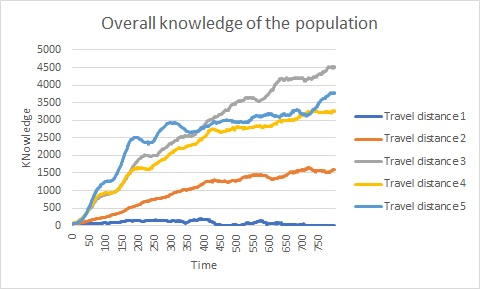
\includegraphics[width=\columnwidth]{KnowledgeGraph}
\caption{Graph showing the knowledge of the population over time}
\end{figure}
\section{Discussion}
As can be seen in Figure 1 as the run distance of each agent increases the total knowledge of the population also increases. However after a run distance of three the total knowledge of the subsequent run distances are lower. This is not what was expected however there are a few reasons that this may be the case for this simulation. The first reason could be that for the size of the world a run distance of three was the most optimal in terms of reaching the largest amount of the population. With increasing run distances the talking agents may have missed more agents that had less knowledge whereas with smaller run distances the agents didn't move far enough to reach the agents with less knowledge. The frequency at which the agents moved was always the same. Testing could be done on varying world sizes as well as different run distances to test if this would be the case. From the \cite{Powell} paper the population density may also be another reason that a run distance of three was the best at transferring knowledge around this population. With larger starting populations of turtles the higher run distances may have more of an effect on the total knowledge as they are more likely to reach a higher number of turtles when moving away from others. Another reason for this may be that the amount of special food was too low and with a higher amount of special food the higher total knowledge will increase with the run distance. Even though the results are not as expected they still show a general trend that the run distance does in fact increase the total knowledge of a population. This is due to agents being able to reach more of the population and as a result the knowledge is spread further around benefiting the whole population. 
\section{Conclusion}
In conclusion this paper simulates using spacial and cognitive agents that the total knowledge of a population is increases if the agents of that population can migrate further. This backs up the conclusion that \cite{Powell} came to and additionally shows that there are many other factors that determine the knowledge of a population. 
\end{multicols}
\newpage
\bibliographystyle{agsm}
\bibliography{bibliography}
\end{document}